\documentclass[11pt]{beamer}
\usepackage[utf8]{inputenc}
\usepackage[T1]{fontenc}
\usepackage{lmodern}
\usepackage[czech]{babel}
\usetheme{metropolis}
\begin{document}
	\author{Lukáš Růžička}
	\title{Jak se zapojit do vývoje svobodného software}
	\subtitle{aneb Ten umí to a ten zas tohle ...}
	%\logo{}
	\institute{lruzicka@redhat.com}
	\date{listopad 2021}
	%\subject{}
	%\setbeamercovered{transparent}
	%\setbeamertemplate{navigation symbols}{}
	\begin{frame}[plain]
		\maketitle
	\end{frame}

\section{Svobodný software a komunita}

 	\begin{frame}{Svobodný software}
 		\textit{Svobodný software} zaručuje svým uživatelům \textbf{čtyři základní svobody}:
 		\begin{enumerate}
 			\item právo program spouštět za jakýmkoliv účelem
 			\item právo zkoumat, jak program funguje, a právo upravit jej pro své účely
 			\item právo šířit kopie programu
 			\item právo šířit upravené verze programu a umožnit komunitě používat tyto úpravy
 		\end{enumerate}
 	\end{frame}
 
 \begin{frame}{Softwarová komunita}
 	
 	\textit{Komunita} je svobodné a zájmové uskupení lidí, kteří jsou sdruženi okolo  \textit{projektu}.
 	
 	\begin{itemize}
 		\item řízená komunita
 		\item spontánní komunita
 	\end{itemize}

 \end{frame}

 \begin{frame}{Řízená komunita}
	
	\textit{Řízená komunita} vznikne, když ji někdo cíleně založí a řídí, aby mohl využívat výhody komunitní spolupráce.
	
	\begin{itemize}
		\item v pozadí může stát firma nebo nadace
		\item implementace firemních způsobů řízení
		\item přísnější pravidla komunity
		\item financování projektu a komunitních akcí
		\item možnost být zaměstnán firmou
		\item riziko korporatizace
		\item přeměna na neřízenou komunitu
	\end{itemize}
\end{frame}

\begin{frame}{Spontánní komunita}
	
	\textit{Spontánní komunita} vznikne sama od sebe na základě kvalitního a~zajímavého projektu.
	
	\begin{itemize}
		\item na počátku stojí jednotlivec, který zveřejní zajímavý projekt
		\item k němu se přidávají další nadšenci
		\item řízení komunity má zpravidla v rukou autor (zakladatel)
		\item riziko zaniknutí nebo rozpadu komunity
		\item nedostatečné financování projektu
		\item možnost být odkoupen firmou
		\item přeměna na řízenou komunitu
	\end{itemize}
\end{frame}

\begin{frame}{Některá fakta o komunitách}
	Během rozsáhlého výzkumu\footnote{\url{http://opensourcesurvey.org}} v roce 2017 se hledaly odpovědi na následující témata:
	\begin{itemize}
		\item problémy
		\item negativní jevy
		\item co je v projektu důležité
		\item jaký postoj mají zaměstnavatelé k open source
		\item čeho si uživatelé nejvíce cení
	\end{itemize}
\end{frame}	

\begin{frame}{Problémy v open source}
	\begin{center}
		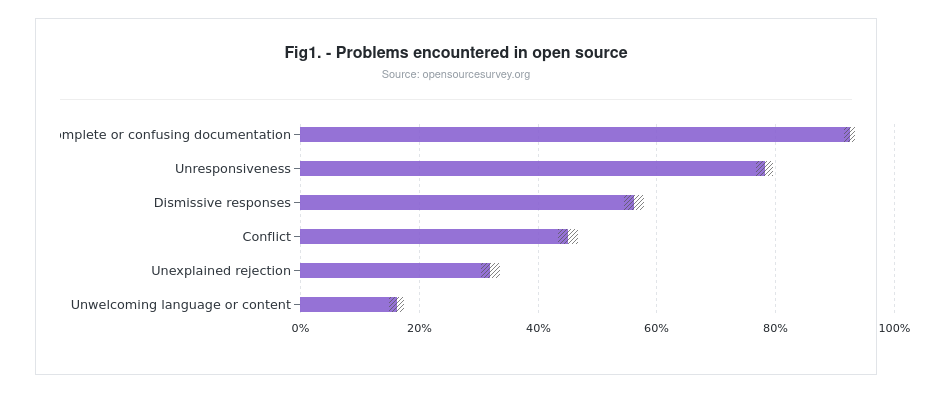
\includegraphics[width=\textwidth]{images/problems.png}
	\end{center}
\end{frame}

\begin{frame}{Negativní jevy v open source}
	\begin{center}
		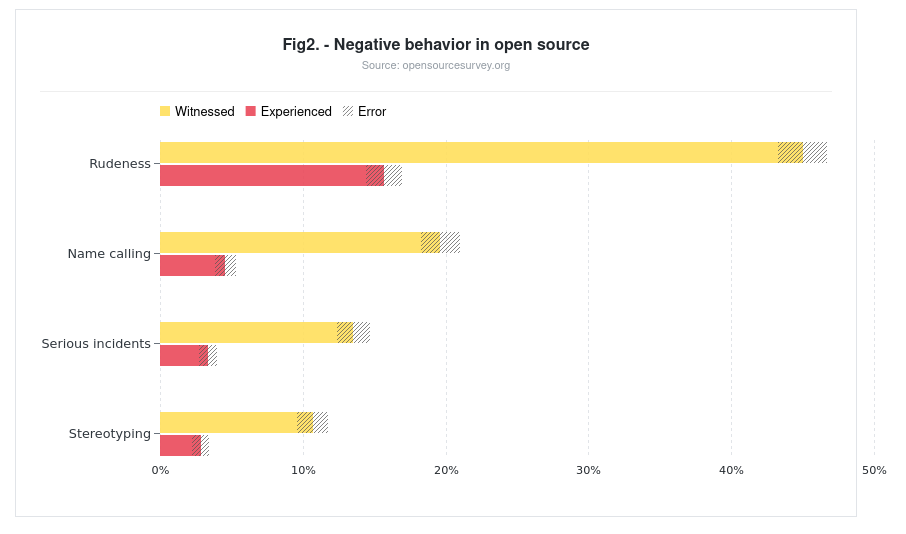
\includegraphics[width=\textwidth]{images/negative_behaviour.png}
	\end{center}
\end{frame}

\begin{frame}{Co je důležité?}
	\begin{center}
		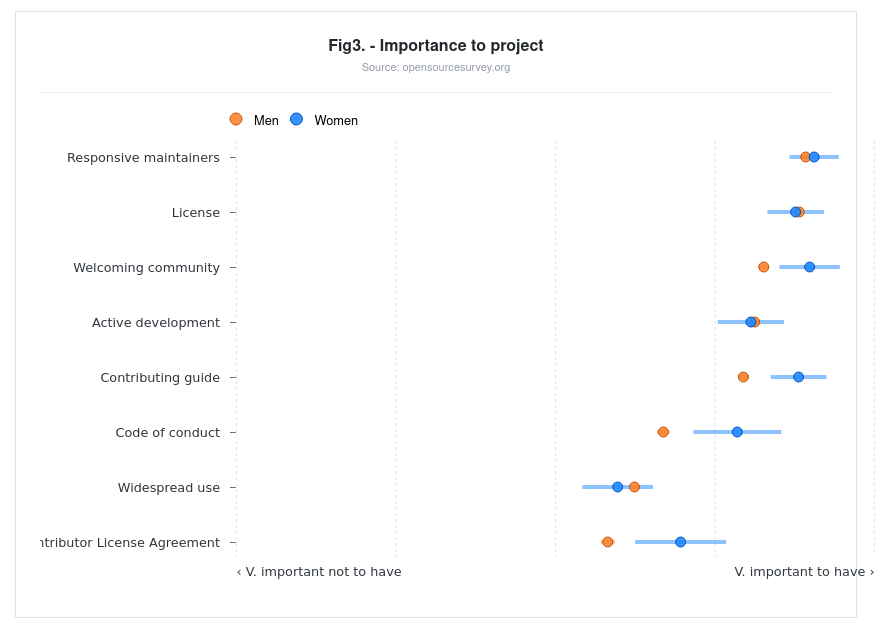
\includegraphics[width=\textwidth]{images/importance.png}
	\end{center}
\end{frame}

\begin{frame}{Jak to vidí zaměstnavatelé?}
	\begin{center}
		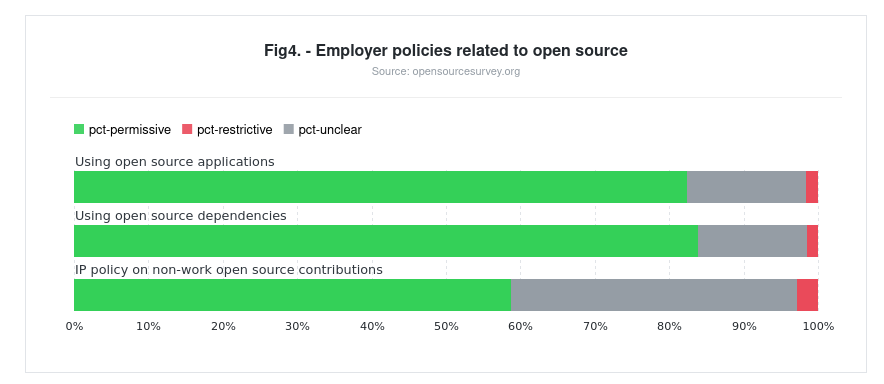
\includegraphics[width=\textwidth]{images/policies.png}
	\end{center}
\end{frame}

\begin{frame}{Čeho si uživatelé cení?}
	\begin{center}
		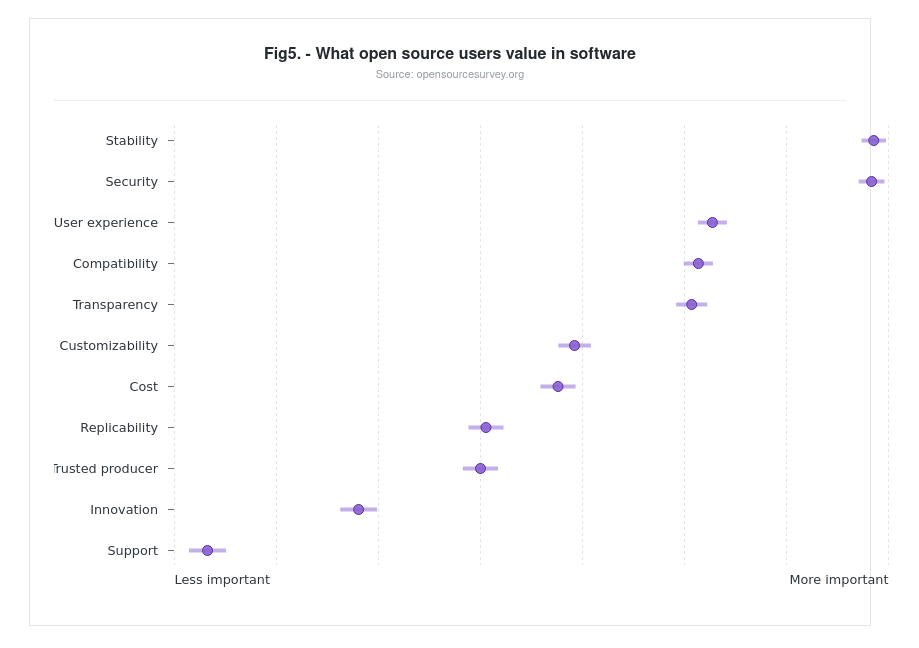
\includegraphics[width=\textwidth]{images/user_value.png}
	\end{center}
\end{frame}

\section{Organizace komunit}

\begin{frame}{Projektové role}	
	\begin{description}
		\item[Author] \hfill \\ zakladatel a \textit{stvořitel} projektu
		\item[Owner]  \hfill \\ vlastník repozitáře nebo organizace spravující projekt
		\item[Maintainers]  \hfill \\ přispěvatelé zodpovědní za projekt, jeho rozvoj, vizi a organizační stránku projektu
		\item[Contributors]  \hfill \\ jednotliví příspěvatelé projektu
		\item[Community Members]  \hfill \\ lidé používající projekt
	\end{description}
\end{frame}

\begin{frame}{Důležité soubory projektu}	
	\begin{description}
		\item[License] \hfill \\ soubor se zněním otevřené licence
		\item[ReadMe]  \hfill \\ základní dokumentace projektu
		\item[Contributing]  \hfill \\ seznam přispěvatelů
		\item[Code of Conduct]  \hfill \\ pravidla chování
	\end{description}
	A některé další. 
\end{frame}

\begin{frame}{Důležité termíny}	
	\begin{description}
		\item[Issue tracker] \hfill \\ systém na sledování problémů
		\item[Pull request]  \hfill \\ žádost o změnu (příspěvek)
		\item[Discussion forum]  \hfill \\ místo, kde se diskutuje o projektu
		\item[Synchronous chat]  \hfill \\ chatovací kanál pro chat v reálném čase
	\end{description}
\end{frame}

\section{Proč a jak přispívat v komunitě?}

 \begin{frame}{Proč lidé přispívají?}
 	\begin{itemize}
 		\item zlepšování software, na kterém  jsou závislí
 		\item zlepšování vlastních profesionálních a osobních dovedností
 		\item setkávání se s podobně naladěnými lidmi
 		\item hledaní mentorů nebo naopak mentorování
 		\item vytváření digitální stopy pro svou profesní reputaci
 		\item učení se \textit{měkkým dovednostem} (people skills)
 		\item vliv na vývoj software
 	\end{itemize}
\end{frame}

 \begin{frame}{Jak lze přispívat?}
	\begin{itemize}
		\item \textbf{není nutné přispívat kódem}
		\item organizační dovednosti
		\item design a grafika
		\item copywriting a psaní dokumentace
		\item plánování komunitních akcí
		\item uživatelská podpora
		\item výuka
		\item překlady
		\item rady a návrhy
		\item finanční podpora
	\end{itemize}
\end{frame}

\section{Jak se přímo zapojit do komunity?}

\begin{frame}{Nebojte se začít}
	\begin{center}
		
\includegraphics[width=\textwidth]{images/multikolo.png} 
		\textit{{\tiny https://opensourcefriday.com/}}
	\end{center}
\end{frame}


\begin{frame}{Komunitní spolupráce}
	
	Aby spolu mohly \textit{globální} komunity efektivně spolupracovat, potřebují nástroj, které jednotlivým příspěvatelům umožní:
	
	\begin{itemize}
		\item lehce získat zdrojové kódy, testovací data, testy, dokumentaci
		\item pracovat na svém počítači s nástroji, na které jsou zvyklí
		\item pracovat na své verzi projektu, aniž by jim do toho někdo zasahoval
		\item snadné ukládání postupu a zálohování na komunitním úložišti
		\item snadné synchronizace s hlavní větví projektů
		\item snadné vytvoření žádosti o změnu (pull request)
		\item kontrola kódu, komentáře, revize, snadný přehled o změnách
		\item snadné převzetí patche (příspěvek) do hlavní verze projektu
	\end{itemize}
\end{frame}

\begin{frame}
	\begin{center}
		{\Huge GitHub!} \\
		\vspace{2cm}
		ale také GitLab, Bitbucket, TaraVault, Sourceforge, Gitbucket, Phabricator, Pagure.
		
	\end{center}
\end{frame}


 \begin{frame}{Potřebné vybavení}
	\begin{itemize}
		\item počítač nebo notebook
		\item přístup na internet
		\item účet na serveru, který komunita používá
		\item editor \textbf{čistého} textu
		\item další software podle potřeby
		\item odhodlanost, trpělivost, toleranci a silné nervy
	\end{itemize}
\end{frame}

 \begin{frame}{Kde mě potřebují?}
 	\textbf{Všude!} Existuje nepřeberné množství projektů, ze kterých si můžete vybrat.
 	
	\begin{itemize}
		\item \url{https://firstcontributions.github.io/}
		\item \url{https://github.com/explore/}
		\item \url{https://www.firsttimersonly.com/}
		\item \url{https://www.codetriage.com/}
		\item \url{https://www.firsttimersonly.com/}
		\item \url{https://24pullrequests.com/}
		\item \url{https://up-for-grabs.net/\#/}
		\item \url{https://contributor.ninja/}
	\end{itemize}
\end{frame}

\begin{frame}{Výběr projektu}
	Při výběru myslete hlavně na to
	\begin{itemize}
		\item jakou roli vlastně chcete dělat
		\item jaký software používáte
		\item s jakými nástroji rádi pracujete
		\item jestli souzníte s filozofií projektu
		\item kolik máte na projekt času
	\end{itemize}
	Dávejte si pozor na to, abyste si vyhradili \textbf{čas na práci} a \textbf{čas na odpočinek}
\end{frame}

\begin{frame}{Jak poznat dobrý projekt?}
	\begin{itemize}
		\item open source
		\item aktivně přijímá příspěvky
		\item otevřený a přístupný
	\end{itemize}
\end{frame}

\begin{frame}{Kdy je open source?}
	Projekt je open source, když je licencovaný pod open source licencí. Licenci často najdeme v souboru \texttt{LICENSE} v kořenovém adresáři projektu.
	
	Některé z otevřených licencí:
	
	\begin{itemize}
		\item  Apache License 2.0
		\item  BSD "Revised" license
		\item  "FreeBSD" license
		\item  GNU General Public License (GPL)
		\item  MIT license
		\item Mozilla Public License 2.0
	\end{itemize}

Více o licencích na \url{https://opensource.org/licenses}.
\end{frame}

\begin{frame}{Kdy aktivně příjímá příspěvky?}
	\begin{itemize}
		\item Kdy byl poslední příspěvek? Kolik příspěvatelů projekt má? Jak často přícházejí příspěvky?
		\item Kolik je otevřených \textit{issues}? Jak dlouho se řeší? Jak často se zavírají a s jakým výsledkem?
		\item Jak je to s \textit{pull requesty}? Diskutuje se o nich aktivně? Jak často se příspěvky vezmou do hlavní větve?
		\item Projekt je \textit{mrtvý}, když v něm není žádná aktivita po dobu nejméně jednoho roku.
	\end{itemize}
\end{frame}

\begin{frame}{Kdy je přístupný?}
	\begin{itemize}
		\item Členové komunity jsou nápomocní.
		\item Jsou přátelští.
		\item Trpělivě odpovídají na otázky.
		\item Komentují a revidují vaše příspěvky.
		\item Poděkují za ně.
	\end{itemize}
\end{frame}


\begin{frame}{Vybrali jsme si projekt.}
	Tak jsme si vybrali svůj první projekt. Co dál?
	\begin{itemize}
		\item \textbf{Používejte jej}.
		\item Testujte.
		\item Komunikujte.
		\item Sledujte informační kanály.
		\item Učte se programovací jazyk projektu a programujte v něm i~vlastní malé věci.
		\item Odevzdejte svůj příspěvek, když jste připraveni.
		\item Neslibujte, co nemůžete splnit.
	\end{itemize}
\end{frame}

\begin{frame}{Jak dát příspěvek?}
	\begin{itemize}
		\item Komunikujte efektivně.
		\item Sbírejte informace.
		\item Nahlašte problém (open an issue).
		\item Otevřete žádost o změnu (open a pull request)
	\end{itemize}
\end{frame}


\begin{frame}{Efektivní komunikace}
	\begin{itemize}
		\item Udělejte si přípravu.
		\item Poskytněte dostatek kontextu.
		\item Pište stručně a k věci.
		\item Komunikujte veřejně.
		\item Ptejte se, ale buďte trpěliví.
		\item Respektujte rozhodnutí komunity.
	\end{itemize}
\end{frame}

\begin{frame}{Sbírání informací}
	\begin{itemize}
		\item dokumentace
		\item issues
		\item pull requests
		\item chatovací kanály
	\end{itemize}
\end{frame}

\begin{frame}{Nahlašte problém}
	Nahlašte problém pokaždé, když
	\begin{itemize}
		\item chcete nahlásit chybu, kterou nemůžete vyřešit sami
		\item chcete diskutovat nápad, vizi, projektovou politiku
		\item navrhnout novou vlastnost 
	\end{itemize}
\end{frame}

\begin{frame}{Komunikujte o problému}

	\begin{itemize}
		\item Neduplikujte problém, pokud víte, že už je nahlášený.
		\item Dejte vědět, že budete problém řešit (assign).
		\item Pokud problém neumíte vyřešit, napište to co nejdříve.
		\item Zjistíte-li, že nahlášený problém není problém, napište to a problém zavřete.
	\end{itemize}
\end{frame}

\begin{frame}{Jak dát pull request?}
	\begin{itemize}
		\item Pull requesty dávejte pro triviální fixy nebo větší úpravy, které již byly prodiskutovány dopředu.
		\item Forkněte repozitář.
		\item Vytvořte novou větev pro vaši práci.
		\item V commit message uvádějte referenci na existující issue (\textit{closes \#18}).
		\item Pokud se změna týká vizuálu, pošlete screenshoty před a po.
		\item Otestujte pořádně vaši práci. Pokud má projekt testovou sadu, použijte ji.
		\item Dodržujte syntaxi a styl projektu.
	\end{itemize}
\end{frame}

\begin{frame}{Co když mi to nevezmou?}
	Pokud jste správně vykomunikovali způsob řešení a poctivě zapracovali všechny požadavky, je velká šance, že \textbf{příspěvek vezmou}.
	
	Když jste příspěvek vytvořili \textbf{ad hoc}, tedy \uv{z čisté vody}, může se stát, že jej nepřijmou, protože se z nějakého důvodu zrovna nehodí. Dost často se lze dozvědět proč a je možné udělat další úpravy, nebo příspěvek nechat na \textbf{vhodnější dobu}.
\end{frame}	

\begin{frame}{Založte vlastní komunitu}
	Začněte vyvíjet vlastní software a dejte ostatním vědět, že to děláte a že se mohou přidat, budou-li chtít.
	
	Takto se do světa dostal \textbf{linuxový kernel}.
\end{frame}	


\section{Jak se zapojit do vývoje Fedory}

\begin{frame}{What can I do for Fedora?}
	
\begin{quotation}
	Don't ask what Fedora can do for you. Ask what you can do for Fedora. 
	\begin{flushright}
			(J. F. Fedorov)
	\end{flushright}	
\end{quotation}
\end{frame}

\begin{frame}{Kde můžete pomoci}
	\begin{itemize}
		\item designerský tým
		\item programování -- Python, C, Haskell, Java, Scala, JavaScript, Ruby, C++ 
		\item podpora komunity
		\item psaní -- dokumentace, blogování
		\item překlady a internacionalizace
		\item obhajoba -- Fedora Ambassadors
		\item balíčkování
		\item \textbf{testování kvality}
		\item desktop, server, cloud
		\item výuka
	\end{itemize}
\end{frame}

\begin{frame}{Kam jít, když chci pomoci?}
	\url{https://whatcanidoforfedora.org/cs}
\end{frame}

\begin{frame}{Testování Fedory}
	\begin{itemize}
		\item \textbf{Fedora QE team}
		\item ČR, USA, Indie, Kanada, Čína
		\item validační testování
		\item testování aplikací
		\item automatizace testů (OpenQA)
		\item metodika a vývoj testů
	\end{itemize}
\end{frame}

\begin{frame}{Jak začít testovat}
	\begin{itemize}
		\item Vytvořit si účet na FAS.\\
		\url{https://accounts.fedoraproject.org/}
		\item Validační testy \\ \url{https://fedoraproject.org/wiki/QA:Release_validation_test_plan}
		\item Test Day \\
		\url{https://testdays.fedoraproject.org/events}
	\end{itemize}
\end{frame}

\begin{frame}{Proč testovat Fedoru?}
	\begin{itemize}
		\item 5 členů týmu v ČR
		\item ochota pomoci
		\item možnost se vidět osobně
		\item testováním se lze naučit Linux
		\item testy zpracované \textit{krok za krokem}\footnote{https://fedoraproject.org/wiki/QA:Testcase\_upgrade\_dnf\_previous\_workstation}
	\end{itemize}
\end{frame}

 \begin{frame}{Použité zdroje}
	\begin{itemize}
		\item \url{https://opensource.guide/how-to-contribute/}
		\item \url{http://opensourcesurvey.org}
		\item \url{https://opensourcefriday.com/}
		\item \url{https://opensource.org/licenses}
		\item \url{https://fedoraproject.org/wiki/}
	\end{itemize}
\end{frame}


\begin{frame}{Otázky a odpovědi}
	\begin{center}
		{\Huge Čas na otázky} 
	\end{center}
\end{frame}

\end{document}